% Algorithms exercise sheet (English, university CS), with code listings, trace tables and a tikz graph.
% Headings: "Exercise N: Title [P pts]" in bold; parts "a.", "b.", ...
\documentclass[11pt,a4paper]{article}
\usepackage[T1]{fontenc}
\usepackage{lmodern}
\usepackage[margin=2.3cm,top=1.8cm,bottom=1.9cm]{geometry}
\usepackage{amsmath,amssymb}
\usepackage{booktabs}
\usepackage{listings}
\usepackage{tikz}
\usetikzlibrary{arrows.meta}
\usepackage{enumitem}

\setlength{\parindent}{0pt}
\setlist[enumerate,1]{label=\alph*., leftmargin=2em, itemsep=0.35em, topsep=0.3em}
\newcommand{\exercise}[3]{\bigskip\par\noindent\textbf{Exercise #1: #2 [#3 pts]}\par\nopagebreak\smallskip}
\newcommand{\blank}{\rule{0pt}{1.1em}\hspace{1.4em}}
\lstset{language=Python, basicstyle=\ttfamily\small, columns=fullflexible, frame=single, framerule=0.3pt,
        xleftmargin=1.2em, xrightmargin=1.2em, aboveskip=0.4em, belowskip=0.2em}

\begin{document}

% ---- header ---------------------------------------------------------------------------
{\small CS 2200 \textperiodcentered{} Algorithms and Data Structures \hfill Autumn 2026}\\[-0.4em]
\rule{\linewidth}{0.6pt}\\[0.5em]
{\Large\bfseries Exercise Sheet 4}\\[0.4em]
Due: Monday, 17 November 2026, 23:59 \hfill Total: 40 points\\[0.3em]
{\small Arrays are 0-indexed. Integer division is written $\lfloor\cdot\rfloor$.}

% ---- Exercise 1 -----------------------------------------------------------------------
\exercise{1}{Binary search}{8}
Consider the sorted array
\[
A = [3,\ 8,\ 14,\ 21,\ 27,\ 35,\ 42,\ 56,\ 63,\ 71,\ 88]
\]
with indices $0,\dots,10$. Binary search keeps a range $[\mathit{lo}, \mathit{hi}]$ and inspects
$\mathit{mid} = \lfloor(\mathit{lo}+\mathit{hi})/2\rfloor$; it sets $\mathit{lo} = \mathit{mid}+1$ if
$A[\mathit{mid}]$ is smaller than the key and $\mathit{hi} = \mathit{mid}-1$ if it is larger. It stops when
the key is found or when $\mathit{lo} > \mathit{hi}$.
\begin{enumerate}
  \item Trace the search for the key $56$. Fill in the table (one row per iteration). [3 pts]
\end{enumerate}
\begin{center}
\begin{tabular}{c|c|c|c|c}
\toprule
iteration & $\mathit{lo}$ & $\mathit{hi}$ & $\mathit{mid}$ & $A[\mathit{mid}]$ \\
\midrule
1 & 0 & 10 & \blank & \blank \\
2 & \blank & \blank & \blank & \blank \\
3 & \blank & \blank & \blank & \blank \\
4 & \blank & \blank & \blank & \blank \\
\bottomrule
\end{tabular}
\end{center}
\begin{enumerate}[resume]
  \item Now search for the key $30$. Trace the search, state the result and the number of iterations. [3 pts]
  \item What is the largest number of iterations binary search needs on an array of 11 elements? [2 pts]
\end{enumerate}

% ---- Exercise 2 -----------------------------------------------------------------------
\exercise{2}{Shortest paths with Dijkstra}{10}
Run Dijkstra's algorithm on the undirected weighted graph in Figure~1, starting at the node $S$.

\begin{center}
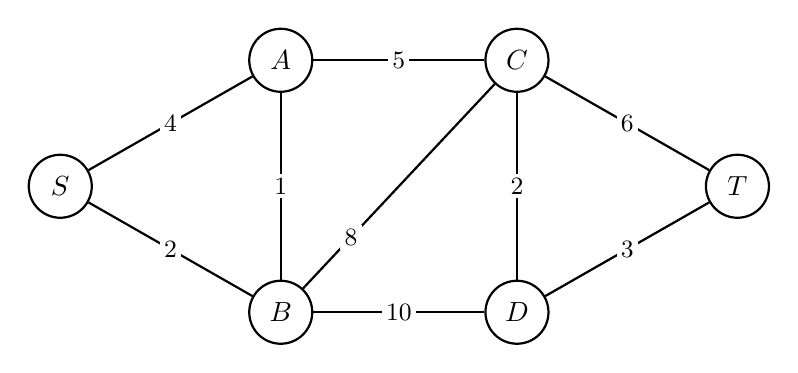
\begin{tikzpicture}[>=Stealth, node distance=2.4cm,
    v/.style={circle, draw, thick, minimum size=0.8cm, inner sep=0pt},
    w/.style={midway, fill=white, inner sep=1.5pt, font=\small}]
  \node[v] (S) at (0,0)    {$S$};
  \node[v] (A) at (2.8,1.6)  {$A$};
  \node[v] (B) at (2.8,-1.6) {$B$};
  \node[v] (C) at (5.8,1.6)  {$C$};
  \node[v] (D) at (5.8,-1.6) {$D$};
  \node[v] (T) at (8.6,0)  {$T$};
  \draw[thick] (S) -- (A) node[w] {4};
  \draw[thick] (S) -- (B) node[w] {2};
  \draw[thick] (A) -- (B) node[w] {1};
  \draw[thick] (A) -- (C) node[w] {5};
  \draw[thick] (B) -- (C) node[pos=0.25, fill=white, inner sep=1.5pt, font=\small] {8};
  \draw[thick] (B) -- (D) node[w] {10};
  \draw[thick] (C) -- (D) node[w] {2};
  \draw[thick] (C) -- (T) node[w] {6};
  \draw[thick] (D) -- (T) node[w] {3};
\end{tikzpicture}

\small Figure 1: Weighted graph with six nodes.
\end{center}
\begin{enumerate}
  \item Make a table with one row per step and write down the current distance estimates of all nodes
        after each step. Mark the node that is finalised in each step. [5 pts]
  \item Give a shortest path from $S$ to $T$ and its length. [2 pts]
  \item Explain why Dijkstra's algorithm can fail on graphs with negative edge weights, and give a
        small example. [3 pts]
\end{enumerate}

% ---- Exercise 3 -----------------------------------------------------------------------
\exercise{3}{Running time of loops}{8}
Give a tight bound $\Theta(\cdot)$ in terms of $n$ for the number of calls to \texttt{work()} and
justify it briefly.
\begin{enumerate}
  \item Snippet 1:
\begin{lstlisting}
for i in range(n):
    for j in range(n):
        work()
\end{lstlisting}
  \item Snippet 2:
\begin{lstlisting}
for i in range(n):
    for j in range(i):
        work()
\end{lstlisting}
  \item Snippet 3:
\begin{lstlisting}
i = 1
while i < n:
    for j in range(n):
        work()
    i = 2 * i
\end{lstlisting}
  \item Snippet 4:
\begin{lstlisting}
i = n
while i >= 1:
    for j in range(i):
        work()
    i = i // 2
\end{lstlisting}
\end{enumerate}

% ---- Exercise 4 -----------------------------------------------------------------------
\exercise{4}{Recurrences and the Master theorem}{6}
Recall: for $T(n) = a\,T(n/b) + f(n)$ with constants $a \ge 1$, $b > 1$, compare $f(n)$ with
$n^{\log_b a}$. Solve the following recurrences with the Master theorem and name the case that applies.
\begin{enumerate}
  \item $T(n) = 4\,T(n/2) + n$
  \item $T(n) = 2\,T(n/2) + n$
  \item $T(n) = 3\,T(n/4) + n^2$
\end{enumerate}

% ---- Exercise 5 -----------------------------------------------------------------------
\exercise{5}{Tracing Python code}{8}
Consider the two functions
\begin{lstlisting}
def mystery(a):
    s = 0
    for x in a:
        if x % 2 == 0:
            s += x
        else:
            s -= 1
    return s

def f(n):
    if n <= 1:
        return 1
    return f(n - 1) + f(n - 2)
\end{lstlisting}
\begin{enumerate}
  \item What does \texttt{mystery([3, 4, 7, 10, 6])} return? Give the value of \texttt{s} after each
        iteration of the loop. [2 pts]
  \item What does \texttt{f(5)} return? [2 pts]
  \item How many calls to \texttt{f} (including the first one) are made when evaluating \texttt{f(4)}? [2 pts]
  \item Give an upper bound on the running time of \texttt{f(n)} and explain why the function is
        inefficient. [2 pts]
\end{enumerate}

\end{document}
